% Options for packages loaded elsewhere
\PassOptionsToPackage{unicode}{hyperref}
\PassOptionsToPackage{hyphens}{url}
\PassOptionsToPackage{dvipsnames,svgnames,x11names}{xcolor}
%
\documentclass[
  letterpaper,
  DIV=11,
  numbers=noendperiod]{scrreport}

\usepackage{amsmath,amssymb}
\usepackage{iftex}
\ifPDFTeX
  \usepackage[T1]{fontenc}
  \usepackage[utf8]{inputenc}
  \usepackage{textcomp} % provide euro and other symbols
\else % if luatex or xetex
  \usepackage{unicode-math}
  \defaultfontfeatures{Scale=MatchLowercase}
  \defaultfontfeatures[\rmfamily]{Ligatures=TeX,Scale=1}
\fi
\usepackage{lmodern}
\ifPDFTeX\else  
    % xetex/luatex font selection
\fi
% Use upquote if available, for straight quotes in verbatim environments
\IfFileExists{upquote.sty}{\usepackage{upquote}}{}
\IfFileExists{microtype.sty}{% use microtype if available
  \usepackage[]{microtype}
  \UseMicrotypeSet[protrusion]{basicmath} % disable protrusion for tt fonts
}{}
\makeatletter
\@ifundefined{KOMAClassName}{% if non-KOMA class
  \IfFileExists{parskip.sty}{%
    \usepackage{parskip}
  }{% else
    \setlength{\parindent}{0pt}
    \setlength{\parskip}{6pt plus 2pt minus 1pt}}
}{% if KOMA class
  \KOMAoptions{parskip=half}}
\makeatother
\usepackage{xcolor}
\setlength{\emergencystretch}{3em} % prevent overfull lines
\setcounter{secnumdepth}{-\maxdimen} % remove section numbering
% Make \paragraph and \subparagraph free-standing
\ifx\paragraph\undefined\else
  \let\oldparagraph\paragraph
  \renewcommand{\paragraph}[1]{\oldparagraph{#1}\mbox{}}
\fi
\ifx\subparagraph\undefined\else
  \let\oldsubparagraph\subparagraph
  \renewcommand{\subparagraph}[1]{\oldsubparagraph{#1}\mbox{}}
\fi

\usepackage{color}
\usepackage{fancyvrb}
\newcommand{\VerbBar}{|}
\newcommand{\VERB}{\Verb[commandchars=\\\{\}]}
\DefineVerbatimEnvironment{Highlighting}{Verbatim}{commandchars=\\\{\}}
% Add ',fontsize=\small' for more characters per line
\usepackage{framed}
\definecolor{shadecolor}{RGB}{241,243,245}
\newenvironment{Shaded}{\begin{snugshade}}{\end{snugshade}}
\newcommand{\AlertTok}[1]{\textcolor[rgb]{0.68,0.00,0.00}{#1}}
\newcommand{\AnnotationTok}[1]{\textcolor[rgb]{0.37,0.37,0.37}{#1}}
\newcommand{\AttributeTok}[1]{\textcolor[rgb]{0.40,0.45,0.13}{#1}}
\newcommand{\BaseNTok}[1]{\textcolor[rgb]{0.68,0.00,0.00}{#1}}
\newcommand{\BuiltInTok}[1]{\textcolor[rgb]{0.00,0.23,0.31}{#1}}
\newcommand{\CharTok}[1]{\textcolor[rgb]{0.13,0.47,0.30}{#1}}
\newcommand{\CommentTok}[1]{\textcolor[rgb]{0.37,0.37,0.37}{#1}}
\newcommand{\CommentVarTok}[1]{\textcolor[rgb]{0.37,0.37,0.37}{\textit{#1}}}
\newcommand{\ConstantTok}[1]{\textcolor[rgb]{0.56,0.35,0.01}{#1}}
\newcommand{\ControlFlowTok}[1]{\textcolor[rgb]{0.00,0.23,0.31}{#1}}
\newcommand{\DataTypeTok}[1]{\textcolor[rgb]{0.68,0.00,0.00}{#1}}
\newcommand{\DecValTok}[1]{\textcolor[rgb]{0.68,0.00,0.00}{#1}}
\newcommand{\DocumentationTok}[1]{\textcolor[rgb]{0.37,0.37,0.37}{\textit{#1}}}
\newcommand{\ErrorTok}[1]{\textcolor[rgb]{0.68,0.00,0.00}{#1}}
\newcommand{\ExtensionTok}[1]{\textcolor[rgb]{0.00,0.23,0.31}{#1}}
\newcommand{\FloatTok}[1]{\textcolor[rgb]{0.68,0.00,0.00}{#1}}
\newcommand{\FunctionTok}[1]{\textcolor[rgb]{0.28,0.35,0.67}{#1}}
\newcommand{\ImportTok}[1]{\textcolor[rgb]{0.00,0.46,0.62}{#1}}
\newcommand{\InformationTok}[1]{\textcolor[rgb]{0.37,0.37,0.37}{#1}}
\newcommand{\KeywordTok}[1]{\textcolor[rgb]{0.00,0.23,0.31}{#1}}
\newcommand{\NormalTok}[1]{\textcolor[rgb]{0.00,0.23,0.31}{#1}}
\newcommand{\OperatorTok}[1]{\textcolor[rgb]{0.37,0.37,0.37}{#1}}
\newcommand{\OtherTok}[1]{\textcolor[rgb]{0.00,0.23,0.31}{#1}}
\newcommand{\PreprocessorTok}[1]{\textcolor[rgb]{0.68,0.00,0.00}{#1}}
\newcommand{\RegionMarkerTok}[1]{\textcolor[rgb]{0.00,0.23,0.31}{#1}}
\newcommand{\SpecialCharTok}[1]{\textcolor[rgb]{0.37,0.37,0.37}{#1}}
\newcommand{\SpecialStringTok}[1]{\textcolor[rgb]{0.13,0.47,0.30}{#1}}
\newcommand{\StringTok}[1]{\textcolor[rgb]{0.13,0.47,0.30}{#1}}
\newcommand{\VariableTok}[1]{\textcolor[rgb]{0.07,0.07,0.07}{#1}}
\newcommand{\VerbatimStringTok}[1]{\textcolor[rgb]{0.13,0.47,0.30}{#1}}
\newcommand{\WarningTok}[1]{\textcolor[rgb]{0.37,0.37,0.37}{\textit{#1}}}

\providecommand{\tightlist}{%
  \setlength{\itemsep}{0pt}\setlength{\parskip}{0pt}}\usepackage{longtable,booktabs,array}
\usepackage{calc} % for calculating minipage widths
% Correct order of tables after \paragraph or \subparagraph
\usepackage{etoolbox}
\makeatletter
\patchcmd\longtable{\par}{\if@noskipsec\mbox{}\fi\par}{}{}
\makeatother
% Allow footnotes in longtable head/foot
\IfFileExists{footnotehyper.sty}{\usepackage{footnotehyper}}{\usepackage{footnote}}
\makesavenoteenv{longtable}
\usepackage{graphicx}
\makeatletter
\def\maxwidth{\ifdim\Gin@nat@width>\linewidth\linewidth\else\Gin@nat@width\fi}
\def\maxheight{\ifdim\Gin@nat@height>\textheight\textheight\else\Gin@nat@height\fi}
\makeatother
% Scale images if necessary, so that they will not overflow the page
% margins by default, and it is still possible to overwrite the defaults
% using explicit options in \includegraphics[width, height, ...]{}
\setkeys{Gin}{width=\maxwidth,height=\maxheight,keepaspectratio}
% Set default figure placement to htbp
\makeatletter
\def\fps@figure{htbp}
\makeatother

\KOMAoption{captions}{tableheading}
\titlehead{
  \begin{center}
    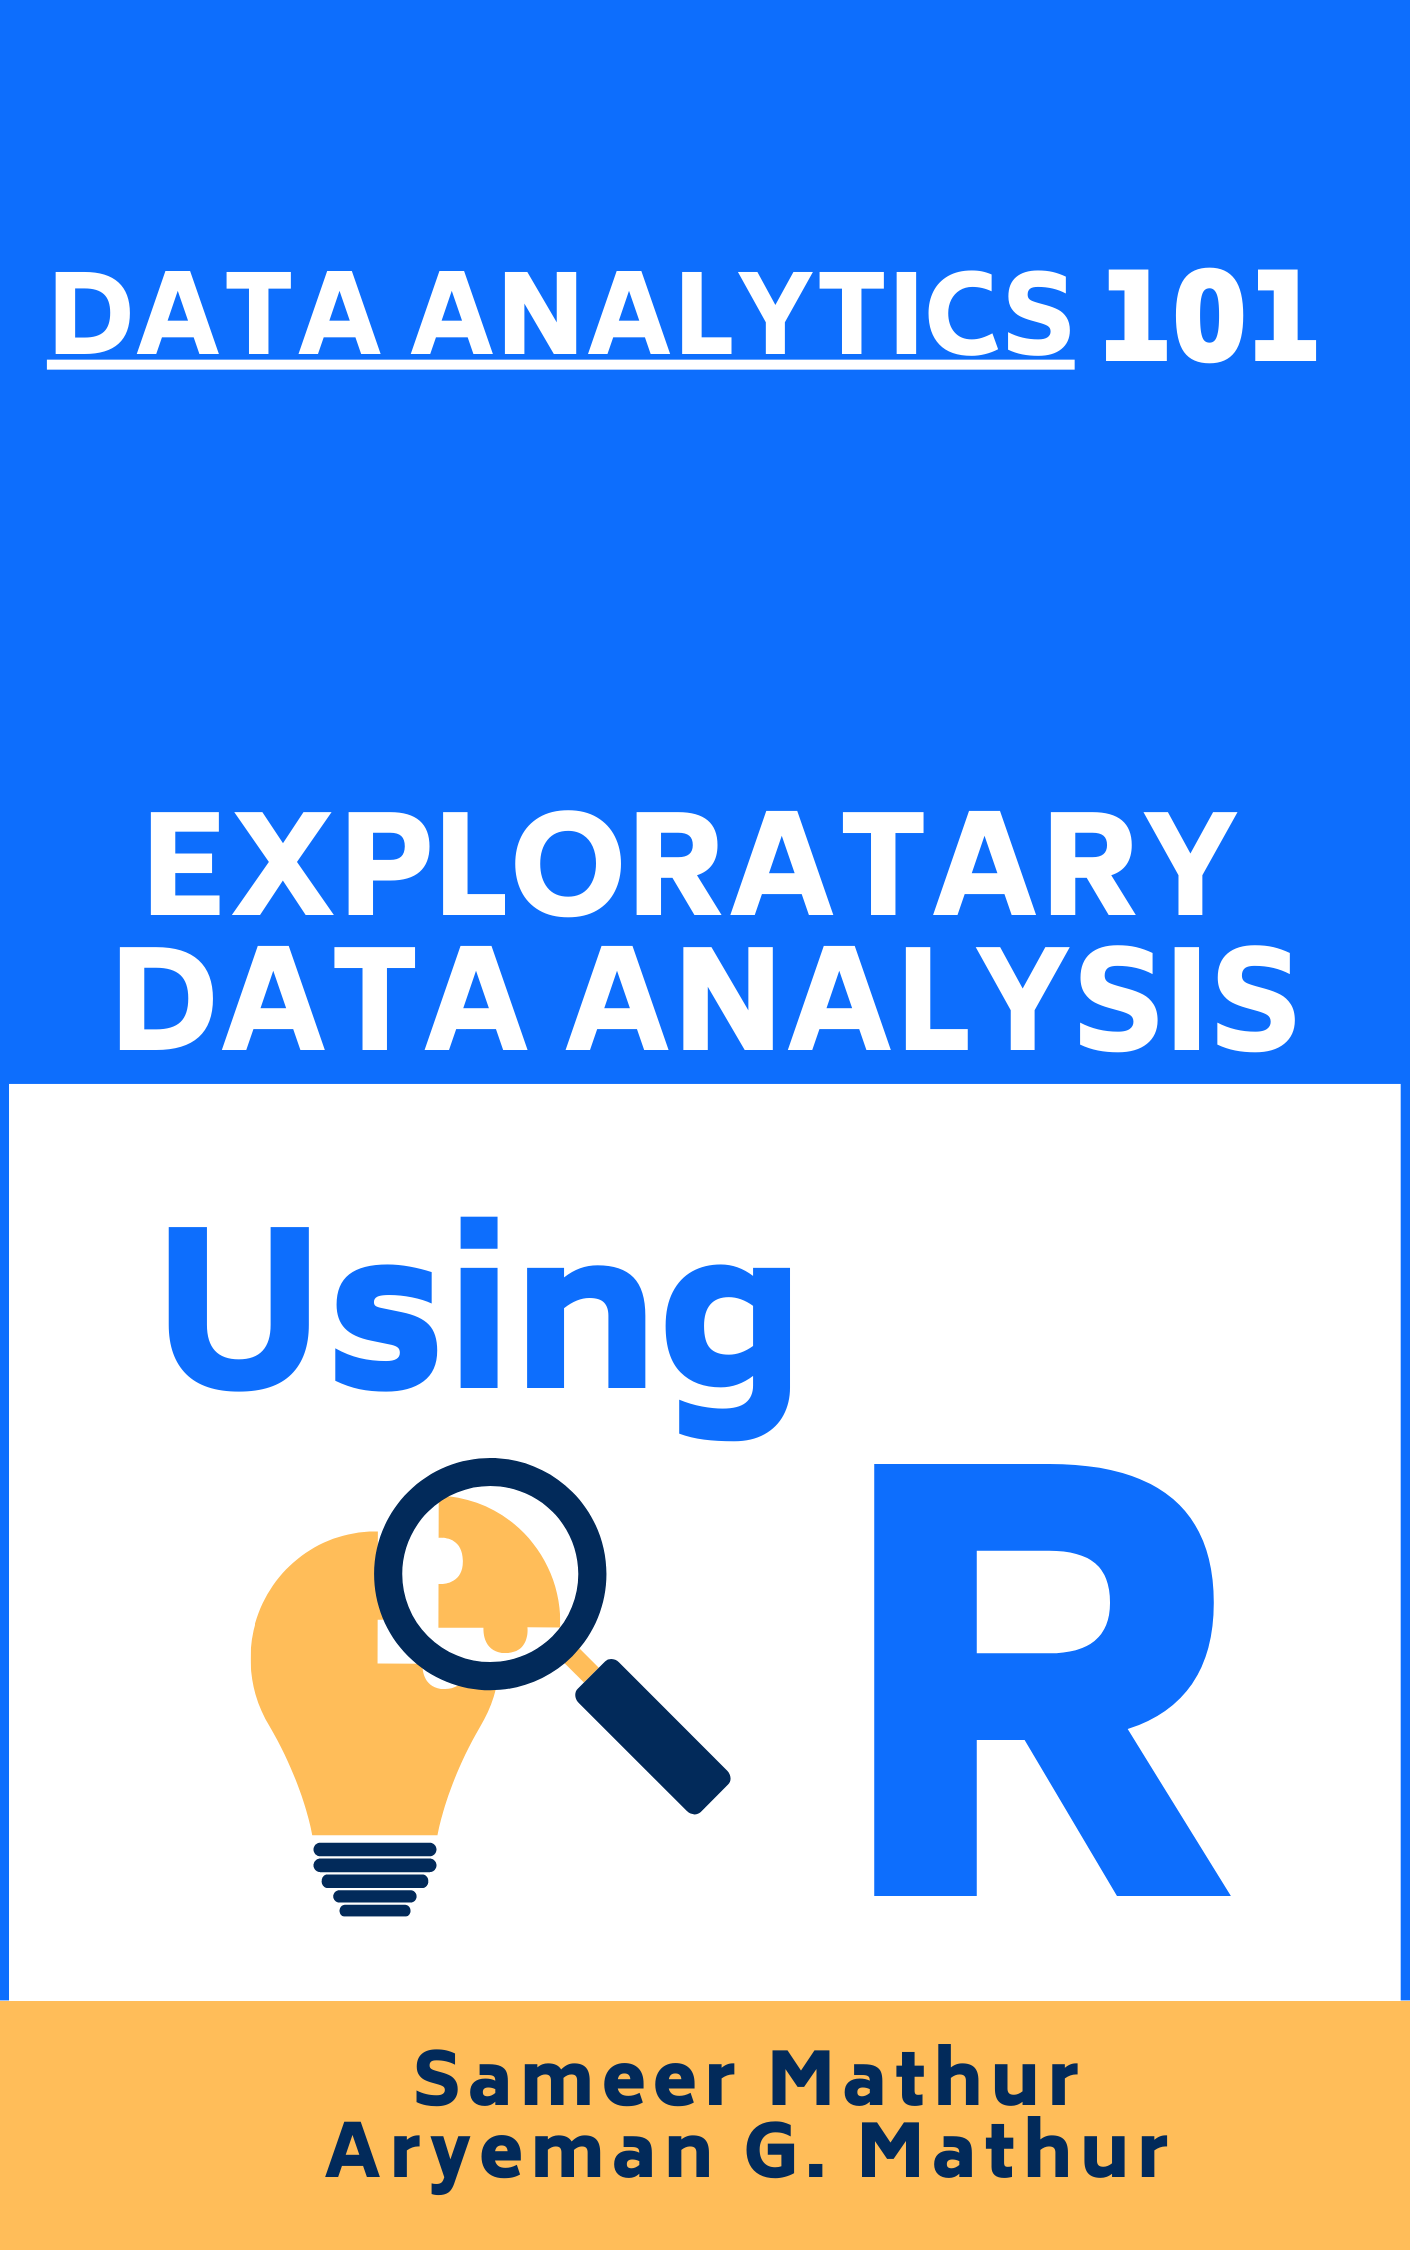
\includegraphics[width=5in]{FINALIZED BOOK COVER.png}
  \end{center}
}
\makeatletter
\makeatother
\makeatletter
\makeatother
\makeatletter
\@ifpackageloaded{caption}{}{\usepackage{caption}}
\AtBeginDocument{%
\ifdefined\contentsname
  \renewcommand*\contentsname{Table of contents}
\else
  \newcommand\contentsname{Table of contents}
\fi
\ifdefined\listfigurename
  \renewcommand*\listfigurename{List of Figures}
\else
  \newcommand\listfigurename{List of Figures}
\fi
\ifdefined\listtablename
  \renewcommand*\listtablename{List of Tables}
\else
  \newcommand\listtablename{List of Tables}
\fi
\ifdefined\figurename
  \renewcommand*\figurename{Figure}
\else
  \newcommand\figurename{Figure}
\fi
\ifdefined\tablename
  \renewcommand*\tablename{Table}
\else
  \newcommand\tablename{Table}
\fi
}
\@ifpackageloaded{float}{}{\usepackage{float}}
\floatstyle{ruled}
\@ifundefined{c@chapter}{\newfloat{codelisting}{h}{lop}}{\newfloat{codelisting}{h}{lop}[chapter]}
\floatname{codelisting}{Listing}
\newcommand*\listoflistings{\listof{codelisting}{List of Listings}}
\makeatother
\makeatletter
\@ifpackageloaded{caption}{}{\usepackage{caption}}
\@ifpackageloaded{subcaption}{}{\usepackage{subcaption}}
\makeatother
\makeatletter
\@ifpackageloaded{tcolorbox}{}{\usepackage[skins,breakable]{tcolorbox}}
\makeatother
\makeatletter
\@ifundefined{shadecolor}{\definecolor{shadecolor}{rgb}{.97, .97, .97}}
\makeatother
\makeatletter
\makeatother
\makeatletter
\makeatother
\ifLuaTeX
  \usepackage{selnolig}  % disable illegal ligatures
\fi
\IfFileExists{bookmark.sty}{\usepackage{bookmark}}{\usepackage{hyperref}}
\IfFileExists{xurl.sty}{\usepackage{xurl}}{} % add URL line breaks if available
\urlstyle{same} % disable monospaced font for URLs
\hypersetup{
  colorlinks=true,
  linkcolor={blue},
  filecolor={Maroon},
  citecolor={Blue},
  urlcolor={Blue},
  pdfcreator={LaTeX via pandoc}}

\author{}
\date{}

\begin{document}
\ifdefined\Shaded\renewenvironment{Shaded}{\begin{tcolorbox}[frame hidden, borderline west={3pt}{0pt}{shadecolor}, interior hidden, sharp corners, breakable, enhanced, boxrule=0pt]}{\end{tcolorbox}}\fi

\hypertarget{categorical-x-categorical-data-1-of-2}{%
\chapter{Categorical x Categorical data (1 of
2)}\label{categorical-x-categorical-data-1-of-2}}

\emph{Dec 30, 2023}

\hypertarget{exploring-bivariate-categorical-data}{%
\section{Exploring Bivariate Categorical
Data}\label{exploring-bivariate-categorical-data}}

This chapter explores how to summarize and visualize \emph{Bivariate,
categorical} data.

\begin{enumerate}
\def\labelenumi{\arabic{enumi}.}
\item
  Bivariate analysis involves examining the \textbf{relationship between
  two variables}. For instance, we might examine the relationship
  between a person's gender (male, female, or non-binary) and whether
  they own a car (yes or no). By exploring these two categorical
  variables together, we can discern potential correlations or
  associations.
\item
  As an extension, multivariate analysis involves the simultaneous
  observation and analysis of more than two variables. We study
  multivariate data in the next chapter.
\item
  \textbf{Contingency Table}: A contingency table, also known as a
  \textbf{cross-tabulation} or \textbf{crosstab}, is a type of table in
  a matrix format that displays the frequency distribution of the
  variables. In the case of a univariate factor variable, a contingency
  table is essentially the same as a frequency table, as there's only
  one variable involved. In more complex analyses involving two or more
  variables, contingency tables provide a way to examine the
  interactions between the variables. {[}1{]}
\item
  \textbf{Data}: Suppose we run the following code to prepare the
  \texttt{mtcars} data for subsequent analysis and save it in a tibble
  called \texttt{tb}.
\end{enumerate}

\begin{Shaded}
\begin{Highlighting}[]
\CommentTok{\# Load the required libraries, suppressing annoying startup messages}
\FunctionTok{library}\NormalTok{(dplyr, }\AttributeTok{quietly =} \ConstantTok{TRUE}\NormalTok{, }\AttributeTok{warn.conflicts =} \ConstantTok{FALSE}\NormalTok{)}
\FunctionTok{library}\NormalTok{(tibble, }\AttributeTok{quietly =} \ConstantTok{TRUE}\NormalTok{, }\AttributeTok{warn.conflicts =} \ConstantTok{FALSE}\NormalTok{)}
\CommentTok{\# Read the mtcars dataset into a tibble called tb}
\FunctionTok{data}\NormalTok{(mtcars)}
\NormalTok{tb }\OtherTok{\textless{}{-}} \FunctionTok{as\_tibble}\NormalTok{(mtcars)}
\CommentTok{\# Convert relevant columns into factor variables}
\NormalTok{tb}\SpecialCharTok{$}\NormalTok{cyl }\OtherTok{\textless{}{-}} \FunctionTok{as.factor}\NormalTok{(tb}\SpecialCharTok{$}\NormalTok{cyl) }\CommentTok{\# cyl = \{4,6,8\}, number of cylinders}
\NormalTok{tb}\SpecialCharTok{$}\NormalTok{am }\OtherTok{\textless{}{-}} \FunctionTok{as.factor}\NormalTok{(tb}\SpecialCharTok{$}\NormalTok{am) }\CommentTok{\# am = \{0,1\}, 0:automatic, 1: manual transmission}
\NormalTok{tb}\SpecialCharTok{$}\NormalTok{vs }\OtherTok{\textless{}{-}} \FunctionTok{as.factor}\NormalTok{(tb}\SpecialCharTok{$}\NormalTok{vs) }\CommentTok{\# vs = \{0,1\}, v{-}shaped engine, 0:no, 1:yes}
\NormalTok{tb}\SpecialCharTok{$}\NormalTok{gear }\OtherTok{\textless{}{-}} \FunctionTok{as.factor}\NormalTok{(tb}\SpecialCharTok{$}\NormalTok{gear) }\CommentTok{\# gear = \{3,4,5\}, number of gears}
\CommentTok{\# Directly access the data columns of tb, without tb$mpg}
\FunctionTok{attach}\NormalTok{(tb)}
\end{Highlighting}
\end{Shaded}

\hypertarget{frequency-tables-for-bivariate-categorical-data}{%
\subsection{Frequency Tables for Bivariate Categorical
Data}\label{frequency-tables-for-bivariate-categorical-data}}

\begin{enumerate}
\def\labelenumi{\arabic{enumi}.}
\item
  As an illustration, let us investigate the bivariate relationship
  between the number of cylinders (\texttt{cyl}) and whether the car has
  an automatic or manual transmission, (\texttt{am=1} for manual,
  \texttt{am=0} for automatic).
\item
  \textbf{\texttt{table()}}: We can use this function to generate a
  contingency table of these two variables.
\end{enumerate}

\begin{Shaded}
\begin{Highlighting}[]
\FunctionTok{table}\NormalTok{(tb}\SpecialCharTok{$}\NormalTok{cyl, tb}\SpecialCharTok{$}\NormalTok{am)}
\end{Highlighting}
\end{Shaded}

\begin{verbatim}
   
     0  1
  4  3  8
  6  4  3
  8 12  2
\end{verbatim}

\begin{itemize}
\item
  In this code, a two-way frequency table of \texttt{am} and
  \texttt{cyl} is created using the \texttt{table()} function. The
  frequency of each grouping of categories is displayed in the table
  that results. As an illustration, there are 8 cars with a manual
  gearbox and 4 cylinders.
\item
  \textbf{\texttt{addmargins()}}: The \texttt{addmargins()} function is
  used to add row and/or column totals to a table.
\end{itemize}

\begin{Shaded}
\begin{Highlighting}[]
\FunctionTok{table}\NormalTok{(tb}\SpecialCharTok{$}\NormalTok{cyl, tb}\SpecialCharTok{$}\NormalTok{am) }\SpecialCharTok{\%\textgreater{}\%} 
  \FunctionTok{addmargins}\NormalTok{()}
\end{Highlighting}
\end{Shaded}

\begin{verbatim}
     
       0  1 Sum
  4    3  8  11
  6    4  3   7
  8   12  2  14
  Sum 19 13  32
\end{verbatim}

\begin{Shaded}
\begin{Highlighting}[]
\FunctionTok{table}\NormalTok{(tb}\SpecialCharTok{$}\NormalTok{cyl, tb}\SpecialCharTok{$}\NormalTok{am) }\SpecialCharTok{\%\textgreater{}\%} 
  \FunctionTok{addmargins}\NormalTok{(}\DecValTok{1}\NormalTok{)}
\end{Highlighting}
\end{Shaded}

\begin{verbatim}
     
       0  1
  4    3  8
  6    4  3
  8   12  2
  Sum 19 13
\end{verbatim}

\begin{itemize}
\tightlist
\item
  In this variation, the \texttt{1} in the function call indicates that
  we want to add \textbf{row totals}. So, this command adds the totals
  (Sum) of each row as a row in the contingency table.
\end{itemize}

\begin{Shaded}
\begin{Highlighting}[]
\FunctionTok{table}\NormalTok{(tb}\SpecialCharTok{$}\NormalTok{cyl, tb}\SpecialCharTok{$}\NormalTok{am) }\SpecialCharTok{\%\textgreater{}\%} 
  \FunctionTok{addmargins}\NormalTok{(}\DecValTok{2}\NormalTok{)}
\end{Highlighting}
\end{Shaded}

\begin{verbatim}
   
     0  1 Sum
  4  3  8  11
  6  4  3   7
  8 12  2  14
\end{verbatim}

\begin{itemize}
\tightlist
\item
  In this variation, the \texttt{2} specifies that we want to add
  \textbf{column totals}. Thus, it adds the totals (Sum) of each column
  to the contingency table.
\end{itemize}

\begin{enumerate}
\def\labelenumi{\arabic{enumi}.}
\setcounter{enumi}{2}
\tightlist
\item
  \textbf{\texttt{xtabs()}}: This function provides a more versatile way
  to generate cross tabulations or contingency tables. It differs from
  the \texttt{table()} function by allowing the use of weights and
  formulas. Here's how we can use it:
\end{enumerate}

\begin{Shaded}
\begin{Highlighting}[]
\FunctionTok{xtabs}\NormalTok{(}\SpecialCharTok{\textasciitilde{}}\NormalTok{ cyl }\SpecialCharTok{+}\NormalTok{ am, }
      \AttributeTok{data =}\NormalTok{ tb)}
\end{Highlighting}
\end{Shaded}

\begin{verbatim}
   am
cyl  0  1
  4  3  8
  6  4  3
  8 12  2
\end{verbatim}

\begin{itemize}
\item
  In the code, we have used \texttt{xtabs()} to construct a
  cross-tabulation of \texttt{am} and \texttt{cyl}.
\item
  The syntax \texttt{\textasciitilde{}\ cyl\ +\ am} is interpreted as a
  formula, signifying that we aim to cross-tabulate these variables. The
  output is a table akin to what we obtain with \texttt{table()}, but
  with the added advantage of accommodating more intricate analyses.
\item
  An important advantage of \texttt{xtabs()} over \texttt{table()} is
  its superior handling of missing values or NAs; it doesn't
  automatically exclude them, which is beneficial when dealing with
  real-world data that often includes missing values. {[}1{]}
\end{itemize}

\begin{enumerate}
\def\labelenumi{\arabic{enumi}.}
\setcounter{enumi}{3}
\tightlist
\item
  \textbf{\texttt{ftable()}}: This function is a powerful tool that
  offers an advanced way to create and display contingency tables.
  Here's an example of its use:
\end{enumerate}

\begin{Shaded}
\begin{Highlighting}[]
\FunctionTok{ftable}\NormalTok{(tb}\SpecialCharTok{$}\NormalTok{cyl, tb}\SpecialCharTok{$}\NormalTok{am)}
\end{Highlighting}
\end{Shaded}

\begin{verbatim}
    0  1
        
4   3  8
6   4  3
8  12  2
\end{verbatim}

\begin{itemize}
\item
  In this code, we've employed the \texttt{ftable()} function to create
  a contingency table of \texttt{am} and \texttt{cyl}. The output of
  this function is similar to what we get using \texttt{table()}, but it
  presents the information in a flat, compact layout, which can be
  particularly helpful especially when dealing with more than two
  variables.
\item
  One key advantage of \texttt{ftable()} is that it creates contingency
  tables in a more readable format when dealing with more than two
  categorical variables, making it easier to visualize and understand
  complex multivariate relationships.
\item
  Do note, like \texttt{xtabs()}, \texttt{ftable()} also handles missing
  values or NAs effectively, making it a reliable choice for real-world
  data that might contain missing values.
\end{itemize}

\begin{enumerate}
\def\labelenumi{\arabic{enumi}.}
\setcounter{enumi}{4}
\tightlist
\item
  We can also use \texttt{group\_by()} and \texttt{summarize()}
  functions from package \texttt{dplyr} to generate contingency tables.
\end{enumerate}

\begin{Shaded}
\begin{Highlighting}[]
\FunctionTok{library}\NormalTok{(dplyr, }\AttributeTok{quietly =} \ConstantTok{TRUE}\NormalTok{, }\AttributeTok{warn.conflicts =} \ConstantTok{FALSE}\NormalTok{)}
\NormalTok{tb }\SpecialCharTok{\%\textgreater{}\%} 
  \FunctionTok{group\_by}\NormalTok{(cyl, am) }\SpecialCharTok{\%\textgreater{}\%}
  \FunctionTok{summarise}\NormalTok{(}\AttributeTok{Frequency =} \FunctionTok{n}\NormalTok{()) }
\end{Highlighting}
\end{Shaded}

\begin{verbatim}
`summarise()` has grouped output by 'cyl'. You can override using the `.groups`
argument.
\end{verbatim}

\begin{verbatim}
# A tibble: 6 x 3
# Groups:   cyl [3]
  cyl   am    Frequency
  <fct> <fct>     <int>
1 4     0             3
2 4     1             8
3 6     0             4
4 6     1             3
5 8     0            12
6 8     1             2
\end{verbatim}

\hypertarget{proportions-table-for-bivariate-categorical-data}{%
\subsection{Proportions Table for Bivariate Categorical
Data}\label{proportions-table-for-bivariate-categorical-data}}

\begin{enumerate}
\def\labelenumi{\arabic{enumi}.}
\setcounter{enumi}{5}
\tightlist
\item
  \textbf{\texttt{prop.table()}}: This function is an advantageous tool
  to understand the relative proportions rather than raw frequencies. It
  converts a contingency table into a table of proportions. Here is how
  we could utilize this function:
\end{enumerate}

\begin{Shaded}
\begin{Highlighting}[]
\NormalTok{freq }\OtherTok{\textless{}{-}} \FunctionTok{table}\NormalTok{(tb}\SpecialCharTok{$}\NormalTok{cyl, tb}\SpecialCharTok{$}\NormalTok{am)}
\NormalTok{prop }\OtherTok{\textless{}{-}} \FunctionTok{prop.table}\NormalTok{(freq)}
\FunctionTok{round}\NormalTok{(prop,}\DecValTok{3}\NormalTok{)}
\end{Highlighting}
\end{Shaded}

\begin{verbatim}
   
        0     1
  4 0.094 0.250
  6 0.125 0.094
  8 0.375 0.062
\end{verbatim}

\begin{itemize}
\item
  In this code, we first generate a frequency table with the
  \texttt{table()} function, using \texttt{cyl} and \texttt{am} as our
  variables. Then, we employ the \texttt{prop.table()} function to
  convert this frequency table (\texttt{freq\_table}) into a proportions
  table (\texttt{prop\_table}).
\item
  This resulting \texttt{prop\_table} reveals the proportion of each
  combination of \texttt{cyl} and \texttt{am} categories relative to the
  total number of observations. This can provide insightful context,
  allowing us to see how each combination fits into the overall
  distribution. For instance, we could learn what proportion of cars in
  our dataset have 4 cylinders and a manual transmission.
\item
  Here is a more efficient method of writing the above code using the
  pipe operator.
\end{itemize}

\begin{Shaded}
\begin{Highlighting}[]
\FunctionTok{table}\NormalTok{(tb}\SpecialCharTok{$}\NormalTok{cyl, tb}\SpecialCharTok{$}\NormalTok{am) }\SpecialCharTok{\%\textgreater{}\%}
  \FunctionTok{prop.table}\NormalTok{() }\SpecialCharTok{\%\textgreater{}\%} 
  \FunctionTok{round}\NormalTok{(}\DecValTok{3}\NormalTok{)}
\end{Highlighting}
\end{Shaded}

\begin{verbatim}
   
        0     1
  4 0.094 0.250
  6 0.125 0.094
  8 0.375 0.062
\end{verbatim}

\begin{enumerate}
\def\labelenumi{\arabic{enumi}.}
\setcounter{enumi}{6}
\tightlist
\item
  We can alternately use package \texttt{dplyr} to showcase the
  frequency and proportions in tabular form, instead of a contingency
  table.
\end{enumerate}

\begin{Shaded}
\begin{Highlighting}[]
\FunctionTok{library}\NormalTok{(dplyr)}
\NormalTok{tb }\SpecialCharTok{\%\textgreater{}\%}
  \FunctionTok{group\_by}\NormalTok{(cyl, am) }\SpecialCharTok{\%\textgreater{}\%}
  \FunctionTok{summarise}\NormalTok{(}\AttributeTok{Frequency =} \FunctionTok{n}\NormalTok{(), }\AttributeTok{.groups =} \StringTok{"drop"}\NormalTok{) }\SpecialCharTok{\%\textgreater{}\%}
  \FunctionTok{mutate}\NormalTok{(}\AttributeTok{Proportion =}\NormalTok{ Frequency }\SpecialCharTok{/} \FunctionTok{sum}\NormalTok{(Frequency)) }
\end{Highlighting}
\end{Shaded}

\begin{verbatim}
# A tibble: 6 x 4
  cyl   am    Frequency Proportion
  <fct> <fct>     <int>      <dbl>
1 4     0             3     0.0938
2 4     1             8     0.25  
3 6     0             4     0.125 
4 6     1             3     0.0938
5 8     0            12     0.375 
6 8     1             2     0.0625
\end{verbatim}

\begin{itemize}
\item
  In this code, \texttt{group\_by(cyl,\ am)} groups the data by
  \texttt{cyl} and \texttt{am}, \texttt{summarise(Frequency\ =\ n())}
  calculates the frequency for each group, \texttt{.groups\ =\ "drop"}
  drops the grouping structure.
\item
  \texttt{mutate(Proportion\ =\ Frequency\ /\ sum(Frequency))}
  calculates the proportions by dividing each frequency by the total sum
  of frequencies.
\item
  The \texttt{mutate()} function adds a new column to the dataframe,
  keeping the original data intact.
\item
  \textbf{Percentages and Rounding}: If we wanted to display the
  proportions as percentages, we could round-off the proportion up to 4
  decimal places, as follows:
\end{itemize}

\begin{Shaded}
\begin{Highlighting}[]
\FunctionTok{library}\NormalTok{(dplyr)}
\NormalTok{tb }\SpecialCharTok{\%\textgreater{}\%}
  \FunctionTok{group\_by}\NormalTok{(cyl, am) }\SpecialCharTok{\%\textgreater{}\%}
  \FunctionTok{summarise}\NormalTok{(}\AttributeTok{Frequency =} \FunctionTok{n}\NormalTok{(), }\AttributeTok{.groups =} \StringTok{"drop"}\NormalTok{) }\SpecialCharTok{\%\textgreater{}\%}
  \FunctionTok{mutate}\NormalTok{(}\AttributeTok{Percentage =} \DecValTok{100}\SpecialCharTok{*}\FunctionTok{round}\NormalTok{(Frequency }\SpecialCharTok{/} \FunctionTok{sum}\NormalTok{(Frequency), }\DecValTok{4}\NormalTok{))}
\end{Highlighting}
\end{Shaded}

\begin{verbatim}
# A tibble: 6 x 4
  cyl   am    Frequency Percentage
  <fct> <fct>     <int>      <dbl>
1 4     0             3       9.38
2 4     1             8      25   
3 6     0             4      12.5 
4 6     1             3       9.38
5 8     0            12      37.5 
6 8     1             2       6.25
\end{verbatim}

\hypertarget{margins-in-proportions-tables}{%
\subsection{Margins in Proportions
Tables}\label{margins-in-proportions-tables}}

\begin{enumerate}
\def\labelenumi{\arabic{enumi}.}
\item
  Different proportions provide various perspectives on the relationship
  between categorical variables in our dataset. We can calculate the i)
  Proportions for \textbf{Each Cell}; (ii) \textbf{Row-Wise*
  Proportions; (iii)} \textbf{Column-Wise} Proportions. This forms a
  crucial part of exploratory data analysis.
\item
  \textbf{Proportions for Each Cell}: This calculates the ratio of each
  cell to the overall total.
\end{enumerate}

\begin{Shaded}
\begin{Highlighting}[]
\FunctionTok{table}\NormalTok{(tb}\SpecialCharTok{$}\NormalTok{cyl, tb}\SpecialCharTok{$}\NormalTok{am) }\SpecialCharTok{\%\textgreater{}\%}
  \FunctionTok{prop.table}\NormalTok{() }\SpecialCharTok{\%\textgreater{}\%} 
  \FunctionTok{addmargins}\NormalTok{() }\SpecialCharTok{\%\textgreater{}\%}
  \FunctionTok{round}\NormalTok{(}\DecValTok{3}\NormalTok{) }\SpecialCharTok{\%\textgreater{}\%}
  \StringTok{\textasciigrave{}}\AttributeTok{*}\StringTok{\textasciigrave{}}\NormalTok{(}\DecValTok{100}\NormalTok{)}
\end{Highlighting}
\end{Shaded}

\begin{verbatim}
     
          0     1   Sum
  4     9.4  25.0  34.4
  6    12.5   9.4  21.9
  8    37.5   6.2  43.8
  Sum  59.4  40.6 100.0
\end{verbatim}

\begin{enumerate}
\def\labelenumi{\arabic{enumi}.}
\setcounter{enumi}{2}
\tightlist
\item
  \textbf{Row-Wise Proportions}: Here, we compute the proportion of each
  cell relative to the total of its row.
\end{enumerate}

\begin{Shaded}
\begin{Highlighting}[]
\FunctionTok{table}\NormalTok{(tb}\SpecialCharTok{$}\NormalTok{cyl, tb}\SpecialCharTok{$}\NormalTok{am) }\SpecialCharTok{\%\textgreater{}\%}
  \FunctionTok{prop.table}\NormalTok{(}\DecValTok{1}\NormalTok{) }\SpecialCharTok{\%\textgreater{}\%} 
  \FunctionTok{addmargins}\NormalTok{(}\DecValTok{2}\NormalTok{) }\SpecialCharTok{\%\textgreater{}\%}
  \FunctionTok{round}\NormalTok{(}\DecValTok{3}\NormalTok{) }\SpecialCharTok{\%\textgreater{}\%}
  \StringTok{\textasciigrave{}}\AttributeTok{*}\StringTok{\textasciigrave{}}\NormalTok{(}\DecValTok{100}\NormalTok{)}
\end{Highlighting}
\end{Shaded}

\begin{verbatim}
   
        0     1   Sum
  4  27.3  72.7 100.0
  6  57.1  42.9 100.0
  8  85.7  14.3 100.0
\end{verbatim}

\begin{enumerate}
\def\labelenumi{\arabic{enumi}.}
\setcounter{enumi}{3}
\tightlist
\item
  \textbf{Column-Wise Proportions}: Here, we determine the proportion of
  each cell relative to the total of its column.
\end{enumerate}

\begin{Shaded}
\begin{Highlighting}[]
\FunctionTok{table}\NormalTok{(tb}\SpecialCharTok{$}\NormalTok{cyl, tb}\SpecialCharTok{$}\NormalTok{am) }\SpecialCharTok{\%\textgreater{}\%}
  \FunctionTok{prop.table}\NormalTok{(}\DecValTok{2}\NormalTok{) }\SpecialCharTok{\%\textgreater{}\%} 
  \FunctionTok{addmargins}\NormalTok{(}\DecValTok{1}\NormalTok{) }\SpecialCharTok{\%\textgreater{}\%}
  \FunctionTok{round}\NormalTok{(}\DecValTok{3}\NormalTok{) }\SpecialCharTok{\%\textgreater{}\%}
  \StringTok{\textasciigrave{}}\AttributeTok{*}\StringTok{\textasciigrave{}}\NormalTok{(}\DecValTok{100}\NormalTok{)}
\end{Highlighting}
\end{Shaded}

\begin{verbatim}
     
          0     1
  4    15.8  61.5
  6    21.1  23.1
  8    63.2  15.4
  Sum 100.0 100.0
\end{verbatim}

\hypertarget{visualizing-bivariate-categorical-data}{%
\section{Visualizing Bivariate Categorical
Data}\label{visualizing-bivariate-categorical-data}}

\begin{enumerate}
\def\labelenumi{\arabic{enumi}.}
\item
  \textbf{Grouped Barplots} and \textbf{Stacked Barplots} serve as
  powerful tools for representing and understanding bivariate
  categorical data, where both variables are categorical in nature.
\item
  Grouped Barplots, often referred to as \textbf{side-by-side bar
  plots}, illustrate the relationship between two categorical variables
  by placing bars corresponding to one category of a variable next to
  each other, differentiated by color or pattern. This layout
  facilitates a direct comparison between categories of the second
  variable. Grouped bar plots are particularly effective when we are
  interested in comparing the distribution of a categorical variable
  across different groups
\item
  On the other hand, \textbf{stacked bar plots} present a similar
  relationship between two categorical variables, but rather than
  aligning bars side by side, they stack bars on top of one another.
  This results in a single bar for each category of one variable, with
  the length of different segments in each bar corresponding to the
  counts or proportions of the categories of the other variable. Stacked
  bar plots are advantageous when we're interested in the total size of
  groups as well as the distribution of a variable across groups.
  {[}2{]}
\item
  \textbf{Grouped Barplot}
\end{enumerate}

\begin{Shaded}
\begin{Highlighting}[]
\CommentTok{\# Create a table with count by transmission and number of cylinders}
\NormalTok{freq }\OtherTok{\textless{}{-}} \FunctionTok{table}\NormalTok{(tb}\SpecialCharTok{$}\NormalTok{cyl, tb}\SpecialCharTok{$}\NormalTok{am)}
\NormalTok{freq}
\end{Highlighting}
\end{Shaded}

\begin{verbatim}
   
     0  1
  4  3  8
  6  4  3
  8 12  2
\end{verbatim}

\begin{Shaded}
\begin{Highlighting}[]
\CommentTok{\# Create a Grouped bar plot}
\FunctionTok{barplot}\NormalTok{(freq, }
        \AttributeTok{beside =} \ConstantTok{TRUE}\NormalTok{, }
        \AttributeTok{col =} \FunctionTok{c}\NormalTok{(}\StringTok{"pink"}\NormalTok{, }\StringTok{"lightblue"}\NormalTok{, }\StringTok{"green"}\NormalTok{), }
        \AttributeTok{xlab =} \StringTok{"Transmission"}\NormalTok{, }\AttributeTok{ylab =} \StringTok{"Frequency"}\NormalTok{, }
        \AttributeTok{main =} \StringTok{"Grouped Barplot of Frequency by transmission and cylinders"}\NormalTok{, }
        \AttributeTok{legend.text =} \FunctionTok{rownames}\NormalTok{(freq), }
        \AttributeTok{args.legend =} \FunctionTok{list}\NormalTok{(}\AttributeTok{title =} \StringTok{"Cylinders"}\NormalTok{))}
\end{Highlighting}
\end{Shaded}

\begin{figure}[H]

{\centering 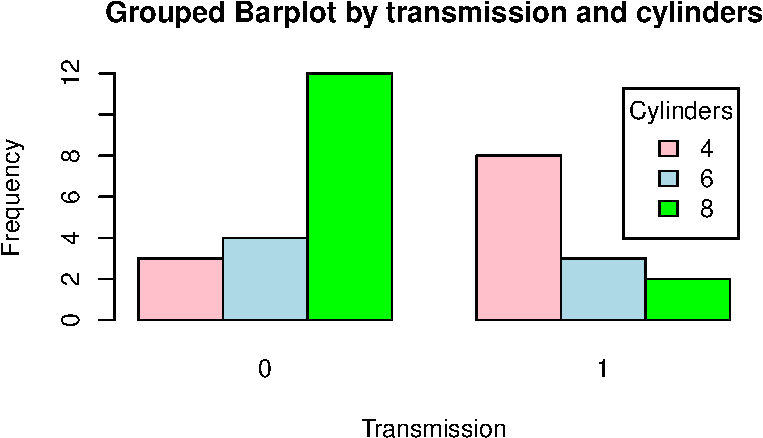
\includegraphics{08CategoricalData02_files/figure-pdf/unnamed-chunk-16-1.pdf}

}

\end{figure}

\begin{enumerate}
\def\labelenumi{\arabic{enumi}.}
\setcounter{enumi}{4}
\tightlist
\item
  \textbf{Discussion}:
\end{enumerate}

\begin{itemize}
\item
  \texttt{freq}: This is the dataset being visualized, which we
  anticipate to be a contingency table of am and cyl variables.
\item
  \texttt{beside} = TRUE: This argument is specifying that the bars
  should be positioned next to each other, which means that for each
  level of \texttt{am}, there will be a distinct bar for each level of
  \texttt{cyl}.
\item
  \texttt{col\ =\ c("pink",\ "lightblue",\ "green")}: Here, we are
  setting the colors of the bars to pink, light blue, and green.
\item
  \texttt{xlab\ =\ "Transmission"} and \texttt{ylab\ =\ "Frequency"}:
  These arguments set the labels for the x and y-axes, respectively.
\item
  \texttt{main} = ``Grouped Barplot of Frequency by transmission and
  cylinders'': This argument assigns a title to the plot.
\item
  \texttt{legend.text\ =\ rownames(freq)}: This creates a legend for the
  plot, using the row names of freq as the legend text.
\item
  \texttt{args.legend\ =\ list(title\ =\ "Cylinders")}: This sets the
  title of the legend to ``Cylinders''.
\end{itemize}

\begin{enumerate}
\def\labelenumi{\arabic{enumi}.}
\setcounter{enumi}{5}
\tightlist
\item
  Consider this alternate barplot.
\end{enumerate}

\begin{Shaded}
\begin{Highlighting}[]
\CommentTok{\# Create a table with count by transmission and number of cylinders}
\NormalTok{freqInverted }\OtherTok{\textless{}{-}} \FunctionTok{table}\NormalTok{(tb}\SpecialCharTok{$}\NormalTok{am, tb}\SpecialCharTok{$}\NormalTok{cyl)}
\NormalTok{freqInverted}
\end{Highlighting}
\end{Shaded}

\begin{verbatim}
   
     4  6  8
  0  3  4 12
  1  8  3  2
\end{verbatim}

\begin{Shaded}
\begin{Highlighting}[]
\CommentTok{\# Create the bar plot}
\FunctionTok{barplot}\NormalTok{(freqInverted, }
        \AttributeTok{beside =} \ConstantTok{TRUE}\NormalTok{, }
        \AttributeTok{col =} \FunctionTok{c}\NormalTok{(}\StringTok{"pink"}\NormalTok{, }\StringTok{"lightblue"}\NormalTok{), }
        \AttributeTok{xlab =} \StringTok{"Cylinders"}\NormalTok{, }\AttributeTok{ylab =} \StringTok{"Count"}\NormalTok{, }
        \AttributeTok{main =} \StringTok{"Grouped Barplot of Frequency by cylinders and transmission"}\NormalTok{, }
        \AttributeTok{legend.text =} \FunctionTok{rownames}\NormalTok{(freqInverted), }
        \AttributeTok{args.legend =} \FunctionTok{list}\NormalTok{(}\AttributeTok{title =} \StringTok{"Transmission"}\NormalTok{))}
\end{Highlighting}
\end{Shaded}

\begin{figure}[H]

{\centering 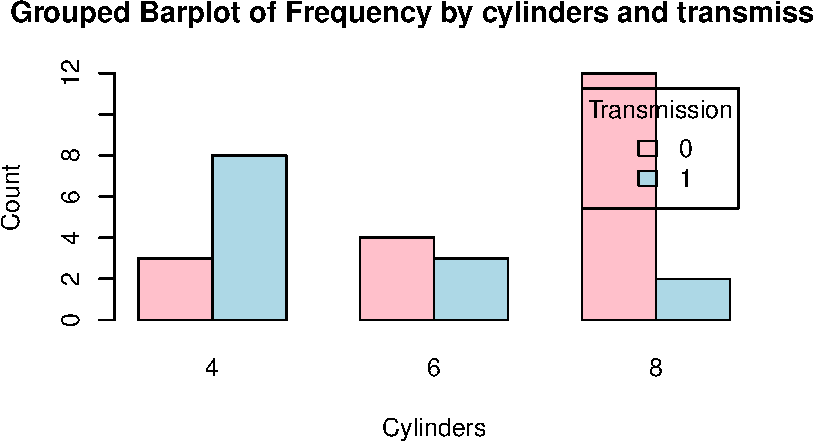
\includegraphics{08CategoricalData02_files/figure-pdf/unnamed-chunk-17-1.pdf}

}

\end{figure}

\begin{enumerate}
\def\labelenumi{\arabic{enumi}.}
\setcounter{enumi}{4}
\tightlist
\item
  \textbf{Discussion}: The most significant differences from the
  previous Grouped Barplot and this one are as follows.
\end{enumerate}

\begin{itemize}
\item
  \texttt{freqInverted}: The contingency table's axes have been swapped
  or inverted. Hence, the table's rows now correspond to the am variable
  (transmission), and its columns correspond to the cyl variable
  (cylinders).
\item
  \texttt{xlab\ =\ "Cylinders"} and \texttt{ylab\ =\ "Count"}: These
  arguments set the labels for the x and y-axes, respectively. This is a
  departure from the previous plot where the x-axis represented
  `Transmission'. In this case, the x-axis corresponds to `Cylinders'.
\item
  \texttt{legend.text\ =\ rownames(freqInverted)} and
  \texttt{args.legend\ =\ list(title\ =\ "Transmission")}: In the
  legend, the roles of `Transmission' and `Cylinders' are reversed
  compared to the previous plot.
\item
  To put it succinctly, the main distinction between the two plots is
  the swapping of the roles of the cyl and am variables. In the second
  plot, `Cylinders' is on the x-axis, which was occupied by
  `Transmission' in the first plot. This perspective shift helps to
  understand the data in a different light, adding another dimension to
  our exploratory data analysis. {[}2{]}
\end{itemize}

\begin{enumerate}
\def\labelenumi{\arabic{enumi}.}
\setcounter{enumi}{4}
\tightlist
\item
  \textbf{Stacked Barplot}
\end{enumerate}

\begin{Shaded}
\begin{Highlighting}[]
\CommentTok{\# Create a table with count by transmission and number of cylinders}
\NormalTok{freq }\OtherTok{\textless{}{-}} \FunctionTok{table}\NormalTok{(tb}\SpecialCharTok{$}\NormalTok{cyl, tb}\SpecialCharTok{$}\NormalTok{am)}
\NormalTok{freq}
\end{Highlighting}
\end{Shaded}

\begin{verbatim}
   
     0  1
  4  3  8
  6  4  3
  8 12  2
\end{verbatim}

\begin{Shaded}
\begin{Highlighting}[]
\CommentTok{\# Create a Stacked bar plot}
\FunctionTok{barplot}\NormalTok{(freq, }
        \AttributeTok{beside =} \ConstantTok{FALSE}\NormalTok{, }
        \AttributeTok{col =} \FunctionTok{c}\NormalTok{(}\StringTok{"pink"}\NormalTok{, }\StringTok{"lightblue"}\NormalTok{, }\StringTok{"green"}\NormalTok{), }
        \AttributeTok{xlab =} \StringTok{"Transmission"}\NormalTok{, }\AttributeTok{ylab =} \StringTok{"Frequency"}\NormalTok{, }
        \AttributeTok{main =} \StringTok{"Stacked Barplot of Frequency by transmission and cylinders"}\NormalTok{, }
        \AttributeTok{legend.text =} \FunctionTok{rownames}\NormalTok{(freq), }
        \AttributeTok{args.legend =} \FunctionTok{list}\NormalTok{(}\AttributeTok{title =} \StringTok{"Cylinders"}\NormalTok{))}
\end{Highlighting}
\end{Shaded}

\begin{figure}[H]

{\centering 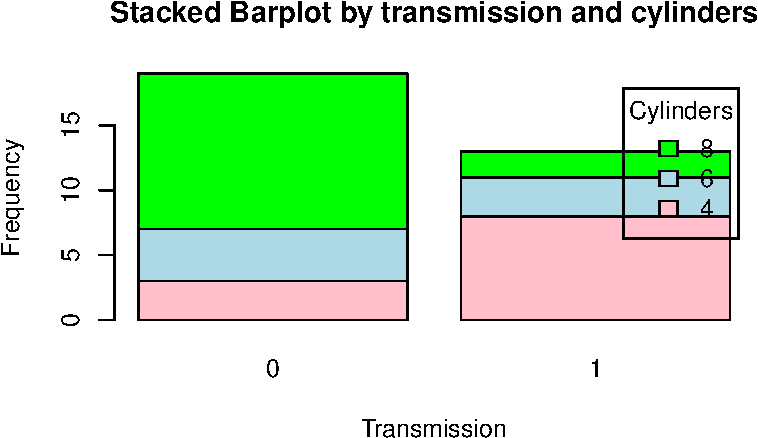
\includegraphics{08CategoricalData02_files/figure-pdf/unnamed-chunk-18-1.pdf}

}

\end{figure}

There are a few key differences between this Stacked Barplot and the
original Grouped Barplot:

\begin{itemize}
\item
  \texttt{beside\ =\ FALSE}: In the original code, beside = TRUE was
  used to generate a grouped bar plot, where each set of bars
  corresponding to each transmission type (automatic or manual) were
  displayed side by side. However, with beside = FALSE, we obtain a
  stacked bar plot. In this plot, the bars corresponding to each
  cylinder category (4, 6, or 8 cylinders) are stacked on top of one
  another for each transmission type.
\item
  \texttt{main\ =\ "Stacked\ Barplot\ of\ Frequency\ by\ transmission\ and\ cylinders"}:
  The title of the plot also reflects this change, mentioning now that
  it's a stacked bar plot instead of a grouped bar plot.
\item
  Finally, here is a Stacked Barplot, corresponding to the second
  Grouped Barplot discussed above.
\end{itemize}

\begin{Shaded}
\begin{Highlighting}[]
\CommentTok{\# Create a table with count by transmission and number of cylinders}
\NormalTok{freqInverted }\OtherTok{\textless{}{-}} \FunctionTok{table}\NormalTok{(tb}\SpecialCharTok{$}\NormalTok{am, tb}\SpecialCharTok{$}\NormalTok{cyl)}
\NormalTok{freqInverted}
\end{Highlighting}
\end{Shaded}

\begin{verbatim}
   
     4  6  8
  0  3  4 12
  1  8  3  2
\end{verbatim}

\begin{Shaded}
\begin{Highlighting}[]
\CommentTok{\# Create the bar plot}
\FunctionTok{barplot}\NormalTok{(freqInverted, }
        \AttributeTok{beside =} \ConstantTok{FALSE}\NormalTok{, }
        \AttributeTok{col =} \FunctionTok{c}\NormalTok{(}\StringTok{"pink"}\NormalTok{, }\StringTok{"lightblue"}\NormalTok{), }
        \AttributeTok{xlab =} \StringTok{"Cylinders"}\NormalTok{, }\AttributeTok{ylab =} \StringTok{"Count"}\NormalTok{, }
        \AttributeTok{main =} \StringTok{"Stacked Barplot of Frequency by cylinders and transmission"}\NormalTok{, }
        \AttributeTok{legend.text =} \FunctionTok{rownames}\NormalTok{(freqInverted), }
        \AttributeTok{args.legend =} \FunctionTok{list}\NormalTok{(}\AttributeTok{title =} \StringTok{"Transmission"}\NormalTok{))}
\end{Highlighting}
\end{Shaded}

\begin{figure}[H]

{\centering 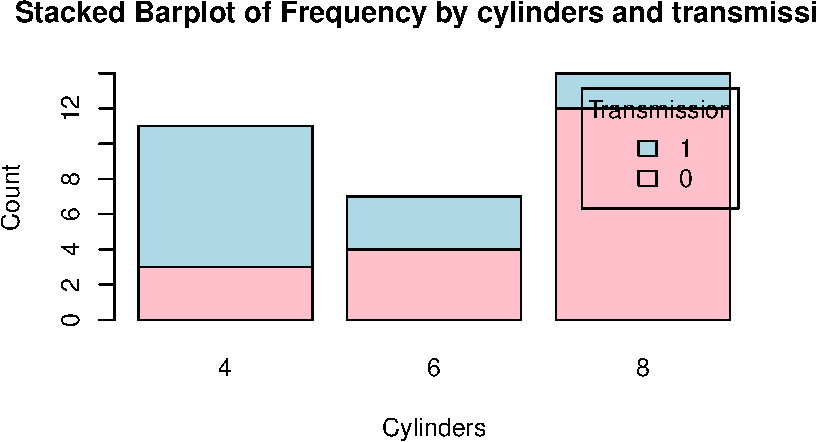
\includegraphics{08CategoricalData02_files/figure-pdf/unnamed-chunk-19-1.pdf}

}

\end{figure}

\begin{enumerate}
\def\labelenumi{\arabic{enumi}.}
\setcounter{enumi}{5}
\tightlist
\item
  The grouped bar plot helps in comparing the number of cylinders across
  transmission types side by side, while the stacked bar plot gives an
  overall comparison in terms of total number of cars, with the
  frequency of each cylinder type stacked on top of the other. The
  choice between a stacked and a grouped bar plot would depend on the
  specific aspects of the data one would want to highlight. Taken
  together, grouped and stacked bar plots offer visually appealing and
  intuitive methods for presenting bivariate categorical data, allowing
  us to understand and analyze relationships between categorical
  variables in a meaningful way. {[}3{]}
\end{enumerate}

\hypertarget{using-ggplot2}{%
\subsection{\texorpdfstring{Using
\textbf{ggplot2}}{Using ggplot2}}\label{using-ggplot2}}

\textbf{Grouped Barplot using ggplot2}

\begin{itemize}
\tightlist
\item
  We demonstrate how to create a Grouped Barplot of Car Count by
  transmission and cylinders
\end{itemize}

\begin{enumerate}
\def\labelenumi{\arabic{enumi}.}
\tightlist
\item
  Set up the data
\end{enumerate}

\begin{Shaded}
\begin{Highlighting}[]
\CommentTok{\# Convert the table to a data frame and reshape to \textquotesingle{}long\textquotesingle{} format}
\NormalTok{freq }\OtherTok{\textless{}{-}} \FunctionTok{table}\NormalTok{(tb}\SpecialCharTok{$}\NormalTok{cyl, tb}\SpecialCharTok{$}\NormalTok{am)}
\NormalTok{df }\OtherTok{\textless{}{-}} \FunctionTok{as.data.frame.table}\NormalTok{(freq)}
\FunctionTok{names}\NormalTok{(df) }\OtherTok{\textless{}{-}} \FunctionTok{c}\NormalTok{(}\StringTok{"Cylinders"}\NormalTok{, }\StringTok{"Transmission"}\NormalTok{, }\StringTok{"Frequency"}\NormalTok{)}
\NormalTok{df}\SpecialCharTok{$}\NormalTok{Cylinders }\OtherTok{\textless{}{-}} \FunctionTok{factor}\NormalTok{(df}\SpecialCharTok{$}\NormalTok{Cylinders)}
\NormalTok{df}\SpecialCharTok{$}\NormalTok{Transmission }\OtherTok{\textless{}{-}} \FunctionTok{factor}\NormalTok{(df}\SpecialCharTok{$}\NormalTok{Transmission, }\AttributeTok{labels =} \FunctionTok{c}\NormalTok{(}\StringTok{"Automatic"}\NormalTok{, }\StringTok{"Manual"}\NormalTok{))}
\end{Highlighting}
\end{Shaded}

\begin{enumerate}
\def\labelenumi{\arabic{enumi}.}
\setcounter{enumi}{1}
\tightlist
\item
  Create a Grouped Barplot using ggplot2
\end{enumerate}

\begin{Shaded}
\begin{Highlighting}[]
\CommentTok{\# Load required library}
\FunctionTok{library}\NormalTok{(ggplot2)}
\end{Highlighting}
\end{Shaded}

\begin{verbatim}

Attaching package: 'ggplot2'
\end{verbatim}

\begin{verbatim}
The following object is masked from 'tb':

    mpg
\end{verbatim}

\begin{Shaded}
\begin{Highlighting}[]
\CommentTok{\# Create the Grouped Barplot}
\FunctionTok{ggplot}\NormalTok{(df, }
       \FunctionTok{aes}\NormalTok{(}\AttributeTok{x =}\NormalTok{ Transmission, }\AttributeTok{y =}\NormalTok{ Frequency, }\AttributeTok{fill =}\NormalTok{ Cylinders)) }\SpecialCharTok{+} 
  \FunctionTok{geom\_bar}\NormalTok{(}\AttributeTok{stat =} \StringTok{"identity"}\NormalTok{, }
           \AttributeTok{position =} \FunctionTok{position\_dodge}\NormalTok{()) }\SpecialCharTok{+}
  \FunctionTok{geom\_text}\NormalTok{(}\FunctionTok{aes}\NormalTok{(}\AttributeTok{label=}\NormalTok{Frequency), }
            \AttributeTok{vjust=}\FloatTok{1.6}\NormalTok{, }
            \AttributeTok{color=}\StringTok{"black"}\NormalTok{, }
            \AttributeTok{position =} \FunctionTok{position\_dodge}\NormalTok{(}\FloatTok{0.9}\NormalTok{), }
            \AttributeTok{size=}\DecValTok{5}\NormalTok{) }\SpecialCharTok{+}
  \FunctionTok{labs}\NormalTok{(}\AttributeTok{x =} \StringTok{"Transmission"}\NormalTok{, }\AttributeTok{y =} \StringTok{"Frequency"}\NormalTok{, }
       \AttributeTok{fill =} \StringTok{"Cylinders"}\NormalTok{,}
       \AttributeTok{title =} \StringTok{"Grouped Barplot of Car Count by transmission and cylinders"}\NormalTok{) }\SpecialCharTok{+}
  \FunctionTok{scale\_fill\_manual}\NormalTok{(}\AttributeTok{values =} \FunctionTok{c}\NormalTok{(}\StringTok{"pink"}\NormalTok{, }\StringTok{"lightblue"}\NormalTok{, }\StringTok{"green"}\NormalTok{))}
\end{Highlighting}
\end{Shaded}

\begin{figure}[H]

{\centering 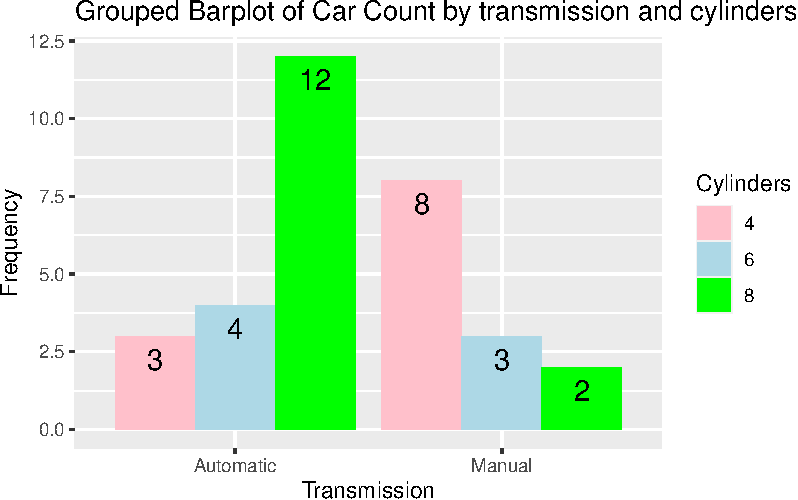
\includegraphics{08CategoricalData02_files/figure-pdf/unnamed-chunk-21-1.pdf}

}

\end{figure}

\begin{enumerate}
\def\labelenumi{\arabic{enumi}.}
\setcounter{enumi}{2}
\tightlist
\item
  \textbf{Discussion}:
\end{enumerate}

\begin{itemize}
\item
  We first convert the frequency table into a data frame that
  \texttt{ggplot2} can use. This involves converting the table to a data
  frame and then reshaping it to long format.
\item
  We then use the \texttt{ggplot()} function to initiate the plot and
  specify the aesthetic mappings. Here, we map `Transmission' to the
  x-axis, `Frequency' to the y-axis, and `Cylinders' to the fill
  aesthetic which controls the color of the bars.
\item
  \texttt{geom\_bar()} with \texttt{stat\ =\ "identity"} is used to add
  the bar geometry to the plot.
\item
  \texttt{position\ =\ position\_dodge()} ensures the bars are placed
  side by side, which creates the grouped effect.
\item
  \texttt{labs()} is used to add labels to the plot.
\item
  \texttt{scale\_fill\_manual()} allows us to manually specify the
  colors for the bars.
\item
  We demonstrate how to create a Grouped Barplot of Car Count by
  cylinders and transmission
\end{itemize}

\begin{enumerate}
\def\labelenumi{\arabic{enumi}.}
\setcounter{enumi}{3}
\tightlist
\item
  Set up the data
\end{enumerate}

\begin{Shaded}
\begin{Highlighting}[]
\NormalTok{freqInverted }\OtherTok{\textless{}{-}} \FunctionTok{table}\NormalTok{(tb}\SpecialCharTok{$}\NormalTok{am, tb}\SpecialCharTok{$}\NormalTok{cyl)}
\CommentTok{\# Convert the table to a data frame and reshape to \textquotesingle{}long\textquotesingle{} format}
\NormalTok{df\_inverted }\OtherTok{\textless{}{-}} \FunctionTok{as.data.frame.table}\NormalTok{(freqInverted)}
\FunctionTok{names}\NormalTok{(df\_inverted) }\OtherTok{\textless{}{-}} \FunctionTok{c}\NormalTok{(}\StringTok{"Transmission"}\NormalTok{, }\StringTok{"Cylinders"}\NormalTok{, }\StringTok{"Count"}\NormalTok{)}
\NormalTok{df\_inverted}\SpecialCharTok{$}\NormalTok{Transmission }\OtherTok{\textless{}{-}} \FunctionTok{factor}\NormalTok{(df\_inverted}\SpecialCharTok{$}\NormalTok{Transmission, }\AttributeTok{labels =} \FunctionTok{c}\NormalTok{(}\StringTok{"Automatic"}\NormalTok{, }\StringTok{"Manual"}\NormalTok{))}
\NormalTok{df\_inverted}\SpecialCharTok{$}\NormalTok{Cylinders }\OtherTok{\textless{}{-}} \FunctionTok{factor}\NormalTok{(df\_inverted}\SpecialCharTok{$}\NormalTok{Cylinders)}
\end{Highlighting}
\end{Shaded}

\begin{enumerate}
\def\labelenumi{\arabic{enumi}.}
\setcounter{enumi}{4}
\tightlist
\item
  Create a Grouped Barplot using ggplot2
\end{enumerate}

\begin{Shaded}
\begin{Highlighting}[]
\CommentTok{\# Create the Grouped Barplot using ggplot2}
\FunctionTok{ggplot}\NormalTok{(df\_inverted, }
       \FunctionTok{aes}\NormalTok{(}\AttributeTok{x =}\NormalTok{ Cylinders, }\AttributeTok{y =}\NormalTok{ Count, }\AttributeTok{fill =}\NormalTok{ Transmission)) }\SpecialCharTok{+} 
  \FunctionTok{geom\_bar}\NormalTok{(}\AttributeTok{stat =} \StringTok{"identity"}\NormalTok{, }
           \AttributeTok{position =} \FunctionTok{position\_dodge}\NormalTok{()) }\SpecialCharTok{+}
  \FunctionTok{geom\_text}\NormalTok{(}\FunctionTok{aes}\NormalTok{(}\AttributeTok{label =}\NormalTok{ Count), }
            \AttributeTok{vjust =} \FloatTok{1.6}\NormalTok{, }
            \AttributeTok{color =} \StringTok{"black"}\NormalTok{, }
            \AttributeTok{position =} \FunctionTok{position\_dodge}\NormalTok{(}\FloatTok{0.9}\NormalTok{), }
            \AttributeTok{size =} \DecValTok{5}\NormalTok{) }\SpecialCharTok{+}
  \FunctionTok{labs}\NormalTok{(}\AttributeTok{x =} \StringTok{"Cylinders"}\NormalTok{, }\AttributeTok{y =} \StringTok{"Count"}\NormalTok{, }\AttributeTok{fill =} \StringTok{"Transmission"}\NormalTok{,}
       \AttributeTok{title =} \StringTok{"Grouped Barplot of Frequency by cylinders and transmission"}\NormalTok{) }\SpecialCharTok{+}
  \FunctionTok{scale\_fill\_manual}\NormalTok{(}\AttributeTok{values =} \FunctionTok{c}\NormalTok{(}\StringTok{"pink"}\NormalTok{, }\StringTok{"lightblue"}\NormalTok{))}
\end{Highlighting}
\end{Shaded}

\begin{figure}[H]

{\centering 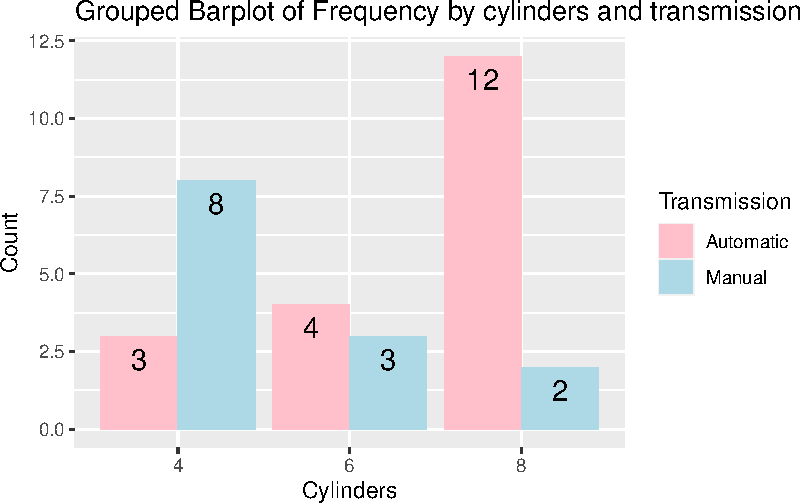
\includegraphics{08CategoricalData02_files/figure-pdf/unnamed-chunk-23-1.pdf}

}

\end{figure}

\begin{enumerate}
\def\labelenumi{\arabic{enumi}.}
\setcounter{enumi}{5}
\tightlist
\item
  \textbf{Discussion}:
\end{enumerate}

\begin{itemize}
\item
  The \texttt{geom\_text()} function is used in the same way as in the
  previous example to add frequency labels to the bars.
\item
  The \texttt{scale\_fill\_manual()} function is used to specify the
  colors for the different transmission types.
\end{itemize}

\textbf{Stacked Barplots using ggplot2}

\begin{itemize}
\item
  We demonstrate how to create a Stacked Barplot of Car Count by
  cylinders and transmission
\item
  To create a stacked bar plot with \texttt{ggplot2}, we apply the
  \texttt{geom\_bar()} function but without the dodge positioning this
  time, since we want the bars stacked.
\end{itemize}

\begin{enumerate}
\def\labelenumi{\arabic{enumi}.}
\setcounter{enumi}{6}
\tightlist
\item
  Create a Stacked Barplot using ggplot2
\end{enumerate}

\begin{Shaded}
\begin{Highlighting}[]
\FunctionTok{library}\NormalTok{(ggplot2)}
\CommentTok{\# Create the Stacked Barplot using ggplot2}
\FunctionTok{ggplot}\NormalTok{(df, }\FunctionTok{aes}\NormalTok{(}\AttributeTok{x =}\NormalTok{ Transmission, }\AttributeTok{y =}\NormalTok{ Frequency, }\AttributeTok{fill =}\NormalTok{ Cylinders)) }\SpecialCharTok{+} 
  \FunctionTok{geom\_bar}\NormalTok{(}\AttributeTok{stat =} \StringTok{"identity"}\NormalTok{) }\SpecialCharTok{+}
  \FunctionTok{geom\_text}\NormalTok{(}\FunctionTok{aes}\NormalTok{(}\AttributeTok{label =}\NormalTok{ Frequency), }
            \AttributeTok{position =} \FunctionTok{position\_stack}\NormalTok{(}\AttributeTok{vjust =} \FloatTok{0.5}\NormalTok{), }
            \AttributeTok{color =} \StringTok{"black"}\NormalTok{, }
            \AttributeTok{size =} \FloatTok{3.5}\NormalTok{) }\SpecialCharTok{+}
  \FunctionTok{labs}\NormalTok{(}\AttributeTok{x =} \StringTok{"Transmission"}\NormalTok{, }\AttributeTok{y =} \StringTok{"Frequency"}\NormalTok{, }
       \AttributeTok{fill =} \StringTok{"Cylinders"}\NormalTok{,}
       \AttributeTok{title =} \StringTok{"Stacked Barplot of Frequency by transmission and cylinders"}\NormalTok{) }\SpecialCharTok{+}
  \FunctionTok{scale\_fill\_manual}\NormalTok{(}\AttributeTok{values =} \FunctionTok{c}\NormalTok{(}\StringTok{"pink"}\NormalTok{, }\StringTok{"lightblue"}\NormalTok{, }\StringTok{"green"}\NormalTok{))}
\end{Highlighting}
\end{Shaded}

\begin{figure}[H]

{\centering 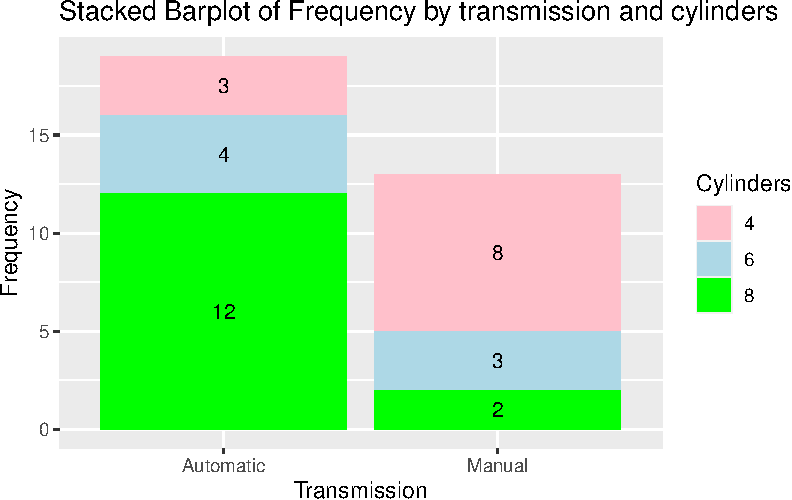
\includegraphics{08CategoricalData02_files/figure-pdf/unnamed-chunk-24-1.pdf}

}

\end{figure}

\begin{enumerate}
\def\labelenumi{\arabic{enumi}.}
\setcounter{enumi}{7}
\tightlist
\item
  \textbf{Discussion}:
\end{enumerate}

\begin{itemize}
\item
  The \texttt{geom\_bar(stat\ =\ "identity")} is used to create a
  stacked bar plot.
\item
  The \texttt{scale\_fill\_manual()} function is used to specify the
  colors for the different cylinder categories. Again, we changed the
  order of the Transmission and Cylinders columns to suit this specific
  plot.
\item
  The \texttt{geom\_text()} function is used to add the labels to the
  stacked bars. We use position\_stack() to position the labels in the
  middle of the stacked sections.
\item
  The \texttt{vjust} argument inside position\_stack() controls the
  vertical positioning of the labels, and 0.5 puts them in the middle.
\item
  As before, \texttt{scale\_fill\_manual()} allows us to specify the
  colors for the different cylinder categories.
\end{itemize}

\hypertarget{mosaic-plots-for-bivariate-categorical-data}{%
\subsection{\texorpdfstring{\textbf{Mosaic Plots} for Bivariate
Categorical
Data}{Mosaic Plots for Bivariate Categorical Data}}\label{mosaic-plots-for-bivariate-categorical-data}}

\begin{enumerate}
\def\labelenumi{\arabic{enumi}.}
\item
  A mosaic plot is a graphical method for visualizing data from two or
  more qualitative variables / categorical data. It is a form of area
  plot that can provide a visual representation of the frequency or
  proportion of the different categories within the variables.
\item
  The following code generates a mosaic plot from a contingency table of
  two variables: \texttt{cyl} (cylinders) and \texttt{am}
  (transmission).
\end{enumerate}

\begin{Shaded}
\begin{Highlighting}[]
\CommentTok{\# Create a mosaic plot }
\FunctionTok{mosaicplot}\NormalTok{(}\FunctionTok{table}\NormalTok{(tb}\SpecialCharTok{$}\NormalTok{cyl, tb}\SpecialCharTok{$}\NormalTok{am), }
           \AttributeTok{main =} \StringTok{"Mosaic of Cylinder count and Transmission type"}\NormalTok{,}
           \AttributeTok{xlab =} \StringTok{"Cylinders (cyl)"}\NormalTok{,}
           \AttributeTok{ylab =} \StringTok{"Transmission (am)"}\NormalTok{)}
\end{Highlighting}
\end{Shaded}

\begin{figure}[H]

{\centering 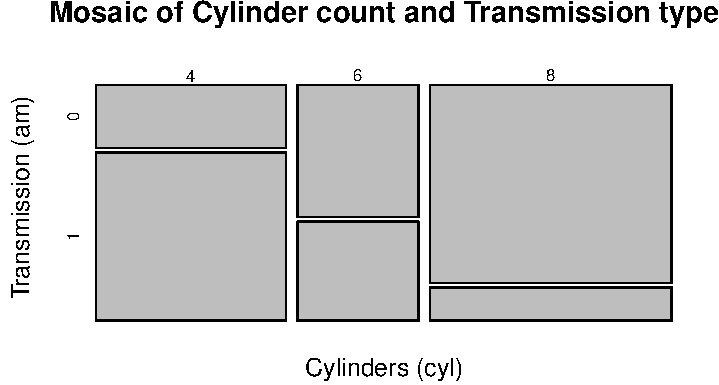
\includegraphics{08CategoricalData02_files/figure-pdf/unnamed-chunk-25-1.pdf}

}

\end{figure}

\begin{enumerate}
\def\labelenumi{\arabic{enumi}.}
\setcounter{enumi}{1}
\tightlist
\item
  In a mosaic plot, we interpret two categorical variables on two axes.
\end{enumerate}

\begin{itemize}
\item
  The \textbf{width} of each section on one axis signifies the
  proportion of that particular category in our dataset.
\item
  Conversely, the \textbf{height} of a section on the other axis
  illustrates the proportion of that category, contingent on the
  specific category from the first variable.
\item
  Therefore, the \textbf{area} of each rectangle directly corresponds to
  the frequency or proportion of observations falling within that
  specific combination of categories (Hartigan \& Kleiner, 1981).
\end{itemize}

\begin{enumerate}
\def\labelenumi{\arabic{enumi}.}
\setcounter{enumi}{2}
\item
  By combining both the height and width of the rectangles, a mosaic
  plot gives us a visual representation of the joint distribution of the
  two categorical variables. It helps us to identify patterns,
  associations, and dependencies between the two variables.
\item
  \textbf{Discussion}:
\end{enumerate}

\begin{itemize}
\item
  The \texttt{table()} function is used to create a contingency table of
  the \texttt{cyl} and \texttt{am} columns of the \texttt{tb} tibble.
  This contingency table represents the counts of all combinations of
  \texttt{cyl} and \texttt{am} in the data.
\item
  The \texttt{mosaicplot()} function then creates a mosaic plot from
  this contingency table. The \texttt{main}, \texttt{xlab}, and
  \texttt{ylab} arguments are used to set the main title, x-axis label,
  and y-axis label of the plot, respectively.
\item
  This code gives a mosaic plot that visualizes the distribution of the
  number of cylinders by the type of transmission. Each block's width in
  the plot would be proportional to the number of cylinders, and the
  height would be proportional to the transmission type.
\end{itemize}

\begin{enumerate}
\def\labelenumi{\arabic{enumi}.}
\setcounter{enumi}{4}
\item
  They can be used to identify breaks in independence or test hypotheses
  regarding the connections between the variables. They are especially
  helpful for examining interactions between two or more categorical
  variables.
\item
  The \texttt{vcd} package, short for Visualizing Categorical Data,
  provides alternative visual and analytical methods for categorical
  data (Meyer, Zeileis, \& Hornik, 2020). A mosaic plot is created from
  the variables \texttt{cyl} (cylinders) and \texttt{am} (transmission
  type) using the \texttt{mosaic()} function.
\end{enumerate}

\begin{Shaded}
\begin{Highlighting}[]
\CommentTok{\# Load the vcd package}
\FunctionTok{library}\NormalTok{(vcd)}
\end{Highlighting}
\end{Shaded}

\begin{verbatim}
Loading required package: grid
\end{verbatim}

\begin{Shaded}
\begin{Highlighting}[]
\CommentTok{\# Create a mosaic plot of mpg (miles per gallon) vs. am (transmission)}
\NormalTok{vcd}\SpecialCharTok{::}\FunctionTok{mosaic}\NormalTok{(}\SpecialCharTok{\textasciitilde{}}\NormalTok{ cyl }\SpecialCharTok{+}\NormalTok{ am, }
       \AttributeTok{data =}\NormalTok{ tb, }
       \AttributeTok{main =} \StringTok{"Mosaic Plot of cars by Cylinder count and Transmission type"}\NormalTok{)}
\end{Highlighting}
\end{Shaded}

\begin{figure}[H]

{\centering 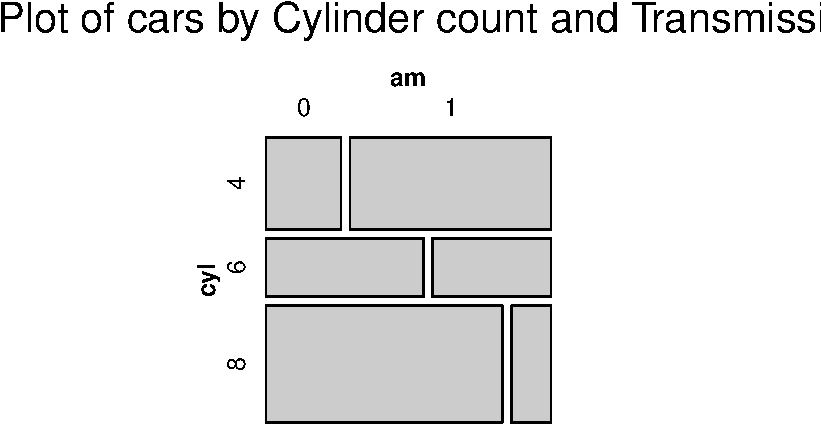
\includegraphics{08CategoricalData02_files/figure-pdf/unnamed-chunk-26-1.pdf}

}

\end{figure}

\begin{enumerate}
\def\labelenumi{\arabic{enumi}.}
\setcounter{enumi}{6}
\tightlist
\item
  \textbf{Discussion}:
\end{enumerate}

\begin{itemize}
\item
  \texttt{library(vcd)} is used to import the vcd package which includes
  the mosaic() function that is superior to the base R mosaicplot() in
  its handling of labeling and legends.
\item
  \texttt{mosaic(\textbackslash{}\textasciitilde{}\ cyl\ +\ am,\ data\ =\ tb,\ main\ =\ "Mosaic\ of\ Cylinder\ count\ and\ Transmission\ type")}
  creates a mosaic plot.
\item
  In this command, the formula \texttt{\textasciitilde{}\ cyl\ +\ am}
  tells R to plot \texttt{cyl} against \texttt{am}. The argument
  \texttt{data\ =\ tb} specifies that the variables for the plot come
  from the \texttt{tb} data frame. The \texttt{main} argument sets the
  title of the plot.
\end{itemize}

\begin{enumerate}
\def\labelenumi{\arabic{enumi}.}
\setcounter{enumi}{7}
\tightlist
\item
  We can customize the shading color of the mosaic plot by setting the
  color using the \texttt{col} argument inside the \texttt{mosaic()}
  function. To specify shades of blue, we can use the
  \texttt{RColorBrewer} package and its \texttt{brewer.pal()} function
  to generate a color palette:
\end{enumerate}

\begin{Shaded}
\begin{Highlighting}[]
\CommentTok{\# Load necessary packages}
\FunctionTok{library}\NormalTok{(vcd)}
\FunctionTok{library}\NormalTok{(RColorBrewer)}

\CommentTok{\# Define the color palette}
\NormalTok{cols }\OtherTok{\textless{}{-}} \FunctionTok{brewer.pal}\NormalTok{(}\DecValTok{4}\NormalTok{, }\StringTok{"Blues"}\NormalTok{)}

\CommentTok{\# Create a mosaic plot}
\NormalTok{vcd}\SpecialCharTok{::}\FunctionTok{mosaic}\NormalTok{(}\SpecialCharTok{\textasciitilde{}}\NormalTok{ cyl }\SpecialCharTok{+}\NormalTok{ am, }
       \AttributeTok{data =}\NormalTok{ tb, }
       \AttributeTok{main =} \StringTok{"Mosaic Plots of cars by Cylinder count and Transmission type"}\NormalTok{,}
       \AttributeTok{shade =} \ConstantTok{TRUE}\NormalTok{,}
       \AttributeTok{highlighting =} \StringTok{"cyl"}\NormalTok{, }
       \AttributeTok{highlighting\_fill =}\NormalTok{ cols)}
\end{Highlighting}
\end{Shaded}

\begin{figure}[H]

{\centering 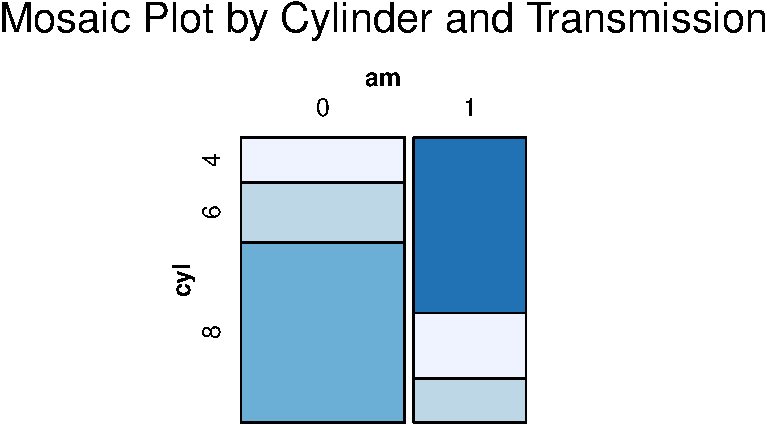
\includegraphics{08CategoricalData02_files/figure-pdf/unnamed-chunk-27-1.pdf}

}

\end{figure}

\begin{enumerate}
\def\labelenumi{\arabic{enumi}.}
\setcounter{enumi}{8}
\tightlist
\item
  \textbf{Discussion}:
\end{enumerate}

\begin{itemize}
\item
  \texttt{brewer.pal(4,\ "Blues")} creates a color palette of 4
  different shades of blue.
\item
  \texttt{highlighting\ =\ "cyl"} means that the shading will
  differentiate the categories in the cyl variable.
\item
  \texttt{highlighting\_fill\ =\ cols} applies the cols color palette to
  the shading.
\end{itemize}

\begin{enumerate}
\def\labelenumi{\arabic{enumi}.}
\setcounter{enumi}{9}
\tightlist
\item
  We can also recreate the previous mosaic plot using \texttt{ggplot2}
  and \texttt{ggmosaic} packages. Here is how to do it:
\end{enumerate}

\begin{Shaded}
\begin{Highlighting}[]
\CommentTok{\# Load the packages}
\FunctionTok{library}\NormalTok{(ggplot2)}
\FunctionTok{library}\NormalTok{(ggmosaic, }\AttributeTok{quietly =} \ConstantTok{TRUE}\NormalTok{, }\AttributeTok{warn.conflicts =} \ConstantTok{FALSE}\NormalTok{)}

\CommentTok{\# Create the mosaic plot}
\FunctionTok{ggplot}\NormalTok{(}\AttributeTok{data =}\NormalTok{ tb) }\SpecialCharTok{+}
  \FunctionTok{geom\_mosaic}\NormalTok{(}\FunctionTok{aes}\NormalTok{(}\AttributeTok{x =} \FunctionTok{product}\NormalTok{(cyl, am), }\AttributeTok{fill =}\NormalTok{ cyl)) }\SpecialCharTok{+}
  \FunctionTok{theme\_minimal}\NormalTok{() }\SpecialCharTok{+}
  \FunctionTok{labs}\NormalTok{(}\AttributeTok{title =} \StringTok{"Mosaic Plot of Cars by Cylinder count and Transmission type"}\NormalTok{, }
       \AttributeTok{x =} \StringTok{"Transmission"}\NormalTok{, }
       \AttributeTok{y =} \StringTok{"Cylinders"}\NormalTok{) }\SpecialCharTok{+}
  \FunctionTok{scale\_fill\_brewer}\NormalTok{(}\AttributeTok{palette =} \StringTok{"Blues"}\NormalTok{)}
\end{Highlighting}
\end{Shaded}

\begin{figure}[H]

{\centering 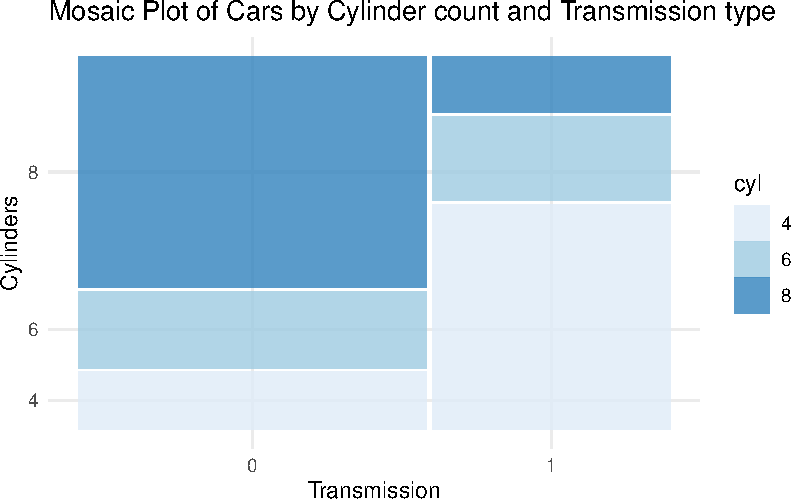
\includegraphics{08CategoricalData02_files/figure-pdf/unnamed-chunk-28-1.pdf}

}

\end{figure}

\begin{enumerate}
\def\labelenumi{\arabic{enumi}.}
\setcounter{enumi}{10}
\tightlist
\item
  \textbf{Discussion}:
\end{enumerate}

\begin{itemize}
\item
  \texttt{geom\_mosaic(aes(x\ =\ product(cyl,\ am),\ fill\ =\ cyl))}
  creates the mosaic plot with \texttt{cyl} and \texttt{am} as the
  categorical variables.
\item
  The \texttt{fill\ =\ cyl} part means that the color fill will
  differentiate the categories in the \texttt{cyl} variable.
\item
  \texttt{theme\_minimal()} applies a minimal theme to the plot.
\item
  \texttt{labs()} is used to specify the labels for the plot, including
  the \texttt{title}, x-axis label, and y-axis label.
\item
  \texttt{scale\_fill\_brewer(palette\ =\ "Blues")} specifies the color
  palette to be used for the fill color, in this case, a palette of
  blues.
\end{itemize}

\hypertarget{summary-of-chapter-9-categorical-x-categorical-data-1-of-2}{%
\section{Summary of Chapter 9 -- Categorical x Categorical data (1 of
2)}\label{summary-of-chapter-9-categorical-x-categorical-data-1-of-2}}

In this chapter, we delve into an extensive exploration of various
methods for visualizing bivariate categorical data using R, which
include but are not limited to grouped bar plots, stacked bar plots, and
mosaic plots.

An explanation is provided to distinguish between grouped and stacked
bar plots, further supported by the inclusion of coding examples and
variations in parameters. Both base R functions and the more advanced
ggplot2 library serve as instrumental tools to depict these techniques,
furnishing readers with a comprehensive understanding of their practical
usage.

The \texttt{ggplot2} library further elevates the possibilities by
offering enhanced customization capabilities and superior control over
aesthetics. Detailed coding examples are presented again to explain both
the grouped and stacked bar plots within this library.

The chapter also introduces mosaic plots as another way of visualizing
bivariate categorical data and discusses how mosaic plots can provide a
visual representation of the frequency or proportion of different
categories within variables. The use of the base R \texttt{mosaicplot()}
function is exemplified, followed by the demonstration of the
\texttt{mosaic()} function in the \texttt{vcd} package and the
\texttt{ggmosaic} package, bringing full circle the spectrum of
visualizations covered for bivariate categorical data.

\hypertarget{references}{%
\section{References}\label{references}}

{[}1{]} Agresti, A. (2018). An Introduction to Categorical Data Analysis
(3rd ed.). Wiley.

Kabacoff, R. I. (2015). R in Action: Data analysis and graphics with R
(2nd ed.). Manning Publications.

Wickham, H., \& Grolemund, G. (2016). R for Data Science: Import, Tidy,
Transform, Visualize, and Model Data. O'Reilly Media.

Hair, J. F., Black, W. C., Babin, B. J., \& Anderson, R. E. (2018).
Multivariate data analysis (8th ed.). Cengage Learning.

{[}2{]} Unwin, A. (2015). Graphical data analysis with R. CRC Press.

Friendly, M. (2000). Visualizing Categorical Data. SAS Institute.

Hartigan, J. A., \& Kleiner, B. (1981). Mosaics for contingency tables.
In Computer Science and Statistics: Proceedings of the 13th Symposium on
the Interface (pp.~268-273).

{[}3{]} Healy, K., \& Lenard, M. T. (2014). A practical guide to
creating better looking plots in R. University of Oregon.
https://escholarship.org/uc/item/07m6r

{[}4{]} Meyer, D., Zeileis, A., \& Hornik, K. (2020). vcd: Visualizing
Categorical Data. R package version 1.4-8.
https://CRAN.R-project.org/package=vcd

Friendly, M. (1994). Mosaic displays for multi-way contingency tables.
Journal of the American Statistical Association, 89(425), 190-200.

Agresti, A. (2018). An Introduction to Categorical Data Analysis (3rd
ed.). Wiley.

{[}5{]} R Core Team (2020). R: A language and environment for
statistical computing. R Foundation for Statistical Computing, Vienna,
Austria. URL https://www.R-project.org/.



\end{document}
